\section{Основное уравнение вращательного движения}

\introProblems

\begin{ex} %Сив313
Найти ускорение грузов и натяжение нитей на машине, изображенной на рис. \ref{AtwoodInertia}, учитывая момент инерции $I$ вращающегося блока, при условии, что нить не скользит по блоку. Определить усилие в подвеске $A$, если масса блока равна $M$.
\begin{ans}
$a= \frac{m_2-m_1}{m_1+m_2+I/r^2}g$, $T_1 = \frac{2m_1m_2g + m_1gI/r^2}{m_1+m_2+I/r^2}$, $T_2 = \frac{2m_1m_2g + m_2gI/r^2}{m_1+m_2+I/r^2}$.
\end{ans}
\end{ex}	

\begin{ex}  %Сив314
Однородный цилиндр массы $M$ и радиуса $R$ (рис. \ref{CylinderInertia}) вращается без трения вокруг горизонтальной оси под действием веса груза $P$, прикрепленного к легкой нити, намотанной на цилиндр. Найти угол $\varphi$ поворота цилиндра в зависимости от времени, если при $t = 0$ $\varphi = 0$.
\begin{ans}
$\varphi = \frac{gt^2}{2R(1+Mg/2P)}$.
\end{ans}
\end{ex}	

\begin{figure}[h]
\centering
\begin{subfigure}{.33\textwidth}
  \centering
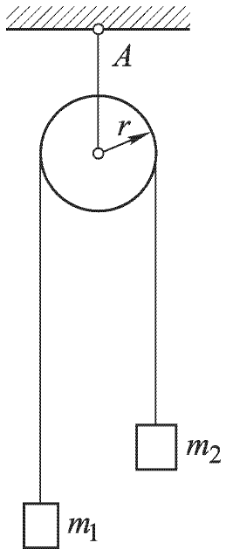
\includegraphics[width=0.6\textwidth]{AtwoodInertia.png}
\caption{}
\label{AtwoodInertia}
\end{subfigure}%
\begin{subfigure}{.33\textwidth}
  \centering
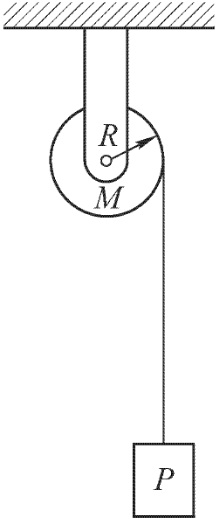
\includegraphics[width=0.6\textwidth]{CylinderInertia.png}
\caption{}
\label{CylinderInertia}
\end{subfigure}
\begin{subfigure}{.33\textwidth}
  \centering
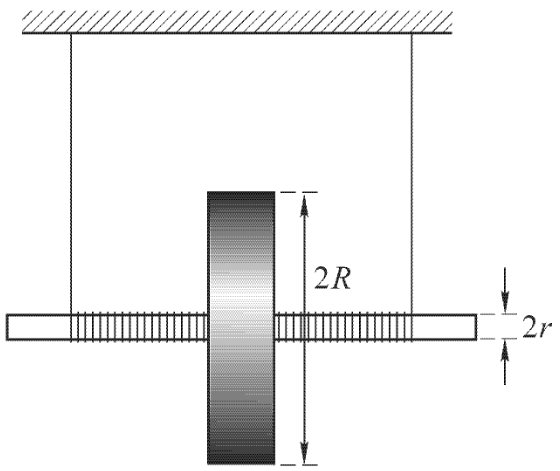
\includegraphics[width=1.2\textwidth]{MaxwellDisk.png}
\caption{}
\label{MaxwellDisk}
\end{subfigure}
\caption{}
\end{figure}

\begin{ex} %Сив319
Схема демонстрационного прибора (диск Максвелла) изображена на рис. \ref{MaxwellDisk}. На валик радиусом $r$ наглухо насажен сплошной диск радиуса $R$ и массы $M$. Валик и диск сделаны из одного материала, причем выступающие из диска части оси имеют массу $m$. К валику прикреплены нити одинаковой длины, при помощи которых прибор подвешивается к штативу. На валик симметрично наматываются нити в один ряд, благодаря чему диск поднимается, а затем предоставляют диску свободно опускаться. Найти ускорение, с которым опускается диск.
\begin{ans}
$a = \frac{2(M+m)r^2}{mr^2+MR^2+2(M+m)r^2}g$.
\end{ans}
\end{ex}	

\begin{ex} %Сив325
По наклонной плоскости, образующей угол $\alpha$ с горизонтом, скатывается без скольжения сплошной однородный диск. Найти линейное ускорение $a$ центра диска.
\begin{ans}
$a=2/3g\sin \alpha$.
\end{ans}
\end{ex}	

\begin{ex} %Сив333
На горизонтальной плоскости лежит катушка ниток. С каким ускорением $a$ будет двигаться ось катушки, если тянуть за нитку с силой $F$ (рис. \ref{Coil})? Каким образом	надо тянуть за нитку, чтобы катушка двигалась в сторону натянутой нитки? Катушка движется по поверхности стола без скольжения. Найти силу трения между катушкой и столом.
\begin{ans}
$a = \frac{F(R\cos \alpha - r)}{I + mR^2}$.
\end{ans}
\end{ex}	

\begin{figure}
\centering
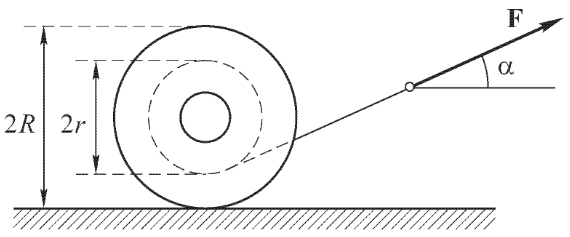
\includegraphics[width=0.5\textwidth]{Coil.png}
\caption{}
\label{Coil}
\end{figure}

\qualProblems

\begin{ex}
Известно, что диск и цилиндр имеют одинаковые массы и радиусы. Каково соотношение их моментов инерции относительно оси симметрии?
\end{ex}	

\begin{ex}
Четыре одинаковых небольших шарика соединили невесомыми стержнями таким образом, что получился квадрат. Во сколько раз момент инерции полученного квадрата относительно одной из сторон больше момента инерции относительно диагонали?
\end{ex}	

\begin{ex}
Какая форма и распределение массы должны быть у маховика, чтобы минимизировать массу и максимизировать момент инерции?
\end{ex}	

\begin{ex}
Цилиндрическое тело массы $m$ и радиуса $R$ имеет неоднородное распределение массы. Может ли масса быть распределенной таким образом, что момент инерции цилиндра относительно оси симметрии превышает $mR^2$? 
\end{ex}	

\simpleProblems

\begin{ex}
Определите момент инерции небольшого карандаша длиной 30 см и массой 50 г относительно оси вращения, перпендикулярной карандашу и проходящей через точку, отстоящую от середины карандаша на 1/6 часть его длины.
\end{ex}	

\begin{ex}
Сплошной диск массой 5 кг и радиусом 0,2 м вращается вокруг оси, перпендикулярной к диску и отстоящей от его центра на 10 см. Чему равен момент инерции диска относительно данной оси вращения?
\end{ex}	

\begin{ex}
В однородном диске массой $m = 1$ кг и радиусом $r = 30$ см вырезано круглое отверстие диаметром $d = 20$ см, центр которого находится на расстоянии $l = 15$ см от оси диска. Найти момент инерции $I$ полученного тела относительно оси, проходящей перпендикулярно плоскости диска через его центр.
\end{ex}	

\begin{ex}
Уравнение вращения шара массой 10 кг и радиусом 20 см вокруг оси, проходящей через его центр имеет вид: $\varphi = 1 + 4t^2 - t^3$. Все величины выражены в СИ. Вычислите вращающий момент, действующий на шар, через 2 с после начала вращения.
\end{ex}	

\begin{ex}
На горизонтальную ось насажены маховик и легкий шкив радиусом $R = 5$ см. На шкив намотан шнур, к которому привязан груз массой $m = 0.4$ кг. Опускаясь равноускорено, груз прошел путь $s = 1.8$ м за время $t = 3$ с. Определить момент инерции $I$ маховика. Массу шкива считать пренебрежимо малой.
\end{ex}	

\complexProblems

\begin{ex} %Сив316
На ступенчатый цилиндрический блок намотаны в противоположных направлениях две легкие нити, нагруженные массами $m_1$ и $m_2$ (рис. \ref{2BlocksInertia}). Найти угловое ускорение блока и натяжения $T_1$ и $T_2$ нитей, учитывая момент инерции $I$ блока.

\begin{figure}[h]
\centering
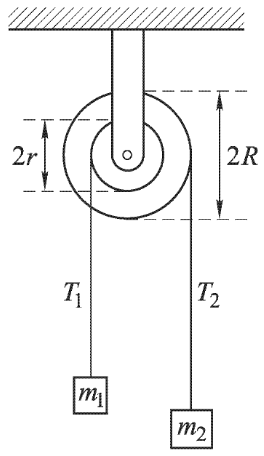
\includegraphics[width=0.25\textwidth]{2BlocksInertia.png}
\caption{}
\label{2BlocksInertia}
\end{figure}

\begin{ans}
$\varepsilon = \frac{m_2R - m_1r}{m_2R^2 + m_1r^2 + I}g$, $T_1 = m_1(g+r\varepsilon)$, $T_2 = m_2(g-R\varepsilon)$.
\end{ans}
\end{ex}	

\begin{ex} %Сив317
Модель ворота укреплена на одной чашке весов (рис. \ref{weighter}). На ворот с моментом инерции $I$ намотана нить с грузиком массы $m$. Весы уравновешены, когда ворот заторможен, и нить не разматывается. Насколько следует изменить вес гирь на другой чашке весов для того, чтобы восстановить равновесие, когда ворот вращается под действием опускающегося вниз грузика?
\begin{ans}
$\Delta m = m/(1+I/mr^2)$.
\end{ans}
\end{ex}	

\begin{figure}[h]
\centering
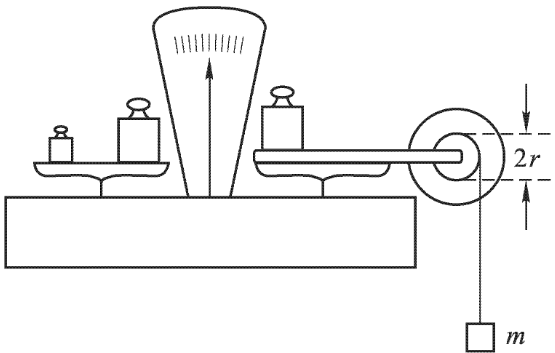
\includegraphics[width=0.4\textwidth]{weighter.png}
\caption{}
\label{weighter}
\end{figure}

\begin{ex} %Сив323
С каким ускорением $a$ будет опускаться катушка с массой $M$ и моментом инерции $I$ относительно оси симметрии, если она подвешена аналогично диску Максвелла (рис. \ref{coil2Threads}). На катушку намотаны еще две нити, к которым подвешен груз массы $m$. Определить натяжения нитей.

\begin{figure}
\centering
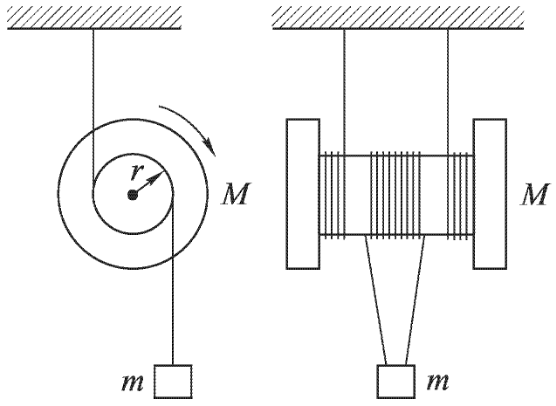
\includegraphics[width=0.4\textwidth]{coil2Threads.png}
\caption{}
\label{coil2Threads}
\end{figure}

\begin{ans}
$a = \frac{M+2m}{4m+M+I/r^2}g$, $T_1 = (2m+I/r^2)a - mg$, $T_2=m(g-2a)$.
\end{ans}
\end{ex}	

\begin{ex} %Сив326
Найти ускорение $a$ центра однородного шара, скатывающегося без скольжения по наклонной плоскости, образующей угол $\alpha$ с горизонтом. Чему равна сила трения сцепления шара и плоскости?
\begin{ans}
$a=5/7g\sin \alpha$.
\end{ans}
\end{ex}	

\begin{ex} %Сив328
По наклонной плоскости, составляющей с горизонтом угол $\alpha = 30^{\circ}$, скатывается без скольжения сплошной однородный цилиндр, масса которого равна 300 г. Найти величину силы трения цилиндра о плоскость.
\begin{ans}
$F = 1/3 mg \sin \alpha$.
\end{ans}
\end{ex}	

\begin{ex} %Сив329
Какова должна быть величина коэффициента трения $\mu$, чтобы однородный цилиндр скатывался без скольжения с наклонной плоскости, образующей угол $\alpha$ с горизонтом?
\begin{ans}
$\mu > 1/3 \tg \alpha$.
\end{ans}
\end{ex}	

\begin{ex} %Сив332
К тележке, стоящей на горизонтальной плоскости, привязана нить, перекинутая через блок, укрепленный у края стола; к концу нити прикреплен груз массы $m_3$ = 500 г. Определить ускорение тележки $a$, если известно, что масса платформы тележки $m_1$ = 1,4 кг, масса каждого колеса $m_2$ = 400 г и колеса представляют собой сплошные диски. Колеса катятся по поверхности стола без скольжения, а трение качения отсутствует.
\begin{ans}
$a = m_3g/(m_1 + 6m_2 +m_3)$.
\end{ans}
\end{ex}	

\clearpage